\documentclass[11pt]{article}
\usepackage{euscript}

\usepackage{amsmath}
\usepackage{amsthm}
\usepackage{amssymb}
\usepackage{epsfig}
\usepackage{xspace}
\usepackage{color}
\usepackage{url}
\usepackage{subfig}
\usepackage{float}
\usepackage{array}
\graphicspath{ {images/} }
%%%%%%%  For drawing trees  %%%%%%%%%
\usepackage{tikz}
\usetikzlibrary{calc, shapes, backgrounds}

%%%%%%%%%%%%%%%%%%%%%%%%%%%%%%%%%
\setlength{\textheight}{9in}
\setlength{\topmargin}{-0.600in}
\setlength{\headheight}{0.2in}
\setlength{\headsep}{0.250in}
\setlength{\footskip}{0.5in}
\flushbottom
\setlength{\textwidth}{6.5in}
\setlength{\oddsidemargin}{0in}
\setlength{\evensidemargin}{0in}
\setlength{\columnsep}{2pc}
\setlength{\parindent}{1em}
%%%%%%%%%%%%%%%%%%%%%%%%%%%%%%%%%


\newcommand{\eps}{\varepsilon}

\renewcommand{\c}[1]{\ensuremath{\EuScript{#1}}}
\renewcommand{\b}[1]{\ensuremath{\mathbb{#1}}}
\newcommand{\s}[1]{\textsf{#1}}
\newcommand{\tb}[1]{\textbf{#1}}

\newcommand{\E}{\textbf{\textsf{E}}}
\renewcommand{\Pr}{\textbf{\textsf{Pr}}}

\title{\textbf{{Question Answering system to effectively answer multiple choice questions using PySpark}}}
%\footnote{\s{CS 6140  Data Mining; \;\; Spring 2015 \hfill
%Instructor: Jeff M. Phillips, University of Utah}
%}

\author{Anirudh Narasimhamurthy(u0941400) and Soumya Smruti Mishra(u0926085)}


\begin{document}
\maketitle
\section{Objective}



\begin{itemize}

\item[] In this part of the assignment we are implementing the Page Rank algorithm for the given data set. Our approach for computing the Page Rank is very similar to the approach specified in Professor's lecture slides.

\textbf{\underline{Data Wrangling/Pre-Processing:}}

\begin {enumerate}

\item The given Wikipedia pages in XML format has several tags for each individual page, but the attributes/tags which we are of interest or importance to us are the $<Title>$, $<Text>$ and the Links within the $<Text>$
 
\item We initially played around with Wiki Parser.py but realized the code it was using wasn't compatible for running on cluster. Also it was not getting all the links from the actual Wikipedia page. So we went around and wrote our own logic for parsing the files.

\item We created a RDD for all the files by reading in the files using sc.wholeTextFiles() and then we applied a map function in which we had our parsing logic.

\item We tweaked the regular expression provided by Hari in the class to make sure it worked for all the content given in these files.

\item We got a list of all the links, list of text content of the file and the title of the page. 

\item\textbf{Return value:} A tuple consisting of  title, (list of links-in-page,text-in-page)

\end{enumerate}

\item We then sorted the list of unique links and enumerated the list of links which in this case would be the title of the n-pages pages in the wiki folder.

\item The transition probability matrix was then constructed as follows:
\begin{enumerate}
	\item The links in the individual page were checked against the global list of links and only those links which were present in global link list were taken into consideration. The appropriate link count was accumulated. The rest of the values were populated as zero.
	
	\item And in case of secondary links of the form $[[A | B]]$, the search was done based on the 'B' value.
	
	\item In cases where there was one or more links to the same page in a single/base page, the sum was accumulated and the final probability values were populated accordingly. For example: If page 1 had 10 outgoing links and 3 of the links were to the same page say Page2, then its corresponding value in matrix would be 0.3 and the other entries would be 0.1 , the sum of which gives us 1.
	
	\item So the transition probability matrix in our case when we did it on 1000 pages wiki data set was a 1000 x 1000 matrix.
\end{enumerate}

\item We also took into consideration the dead-ends and included the taxation parameter while computing the matrix vector product.

\item The expression we used for computing the page Rank was :
\begin{center} $\boxed{v' = \beta M v + \frac{(1- \beta) * e}{n} }$ \end{center}
\begin{itemize}
	\item M : transition probability matrix 
	\item $\beta$ : Taxation parameter (We took it as 0.85).
	\item v : Probability distribution for the location of a random surfer. To start with we took it as 1/n, equal probability of the random surfer being on any of the n-pages.
	\item e : Unit vector
	\item n : number of pages.
\end{itemize} 

\item The computation was done in a simpler way. We first multiplied the matrix entries by the scalar $\beta$ and then added the value of vector $(1- \beta) /n$ to every row of the matrix. In this way we had one matrix and then final operation was to perform the matrix vector multiplication. This note on Page Rank helped us:  \url{http://introcs.cs.princeton.edu/java/16pagerank/}

\item The matrix-vector multiplication was performed in a recursive manner. The resulting vector v' was used as the input v for the next iteration.The threshold or the convergence limit which we took was 0.000001.

\item The threshold limit was computed by taking the second norm of the difference of v and v'.

\item We stored the results of the Page Rank in a dictionary, with title as key and (page Name, index of enumerated link) as the value. We also wrote the results to a json file so that it could be used in the later parts. This is a one-time process and as it was mentioned in the assignment description, we computed and stored them.

\item \textbf{\underline{A note on the results:}} For the smallPages data set, we found the page page-0001960.xml to have the highest page rank value. The title of the page being 'Brazil' and page Rank value being:  6.59559797186e-07.

\end{itemize}

\section{Generating descriptor from the text}

\begin{itemize}
	
	\item[] In this part of the project, we generated the descriptor or the measure of relevance between the text in one page and across the other pages in the given data set or corpus, so that finally when we search for a term, the results displayed are relevant both on the content and the page Rank of the page.
	
	\item The assignment description suggested using Jaccard or cosine similarity to generate the descriptor. As a personal opinion, I realized both of them might not work efficiently without context. 
	
	\item For instance if we were to use cosine similarity based on the most frequent words across all the pages and then build the feature vector and compute the similarity and if the search string or word were to be a word which was not in the list, then our results more or less would have to depend on page Rank which didn't' seem a nice thing to do.
	
	\item So we read about the different approaches which could be used and came across \textbf{TF-IDF} approach which perfectly fits in the description for the assignment.
	
	\item TF-IDF is term frequency-inverse document frequency \url{https://en.wikipedia.org/wiki/Tf–idf} For every page, we first passed the page through our textParsing() function to obtain all the words in cleaned up format from the <text>.
	
	\item The term frequency was then computed for each word in the file. A  couple of \textbf{Spark mllib} functions helped us out.
	
	\item We then computed the inverse term document frequency which is a measure of how much information the word provides, that is, whether the term is common or rare across all documents. If a word appeared several times in one page and did not appear across all the other documents, then it will get a higher value and so when the search term is that word, we would be able to display that page as the first result. If a word was common across all documents, then it would have very low idf value.
	
	\item We then applied appropriate spark functions and stored the results in a form which would be easier for us to retrieve. TF-IDF functions give us a hash value for every word and so we had to do some processing to map the value to the corresponding word and stored them in  a dictionary which would allow a easy look up.
	
	\item We again stored the values in the dictionary to json file, so that it could be used by us for appropriate look up in the search. Sticking with the description provided in the assignment, the descriptors were generated once and stored.
	
	\item{\textbf{Thus the TF-IDF approach worked great for the application and we had a list of all the values for different words and this was one of the parameters which we used to filter and display the search results. Search results displayed would now have the relevance parameter factored in the calculation thanks to this descriptor.}}
	
\end{itemize}

\section{Actual Search}


\begin{enumerate}

\item [] In this part of the assignment, we perform the actual search for the pages.

\item Our search function takes in a search string which could be one or more words and then displays a list of Wikipedia pages from the data set ordered by page rank and relevance of the search term.

\item For a single word search string, our code does a really good job of returning the appropriate results. For single word search string, we felt the relevance or tf-idf value played a much important role than page rank in determining the correctness of the results. So we ordered them first on tf-idf values and then on the page-rank results and the results turned out t be very good.

\item For multiple worded search string, our approach was to actually split the words in search string and store them in a list and then go through each word and finally return pages which had the words appearing in the search term with priority being given to the first and second words in the search string.

\item This might not be the best approach or the neatest way of doing it and at this point in time we are experimenting with the idea of to possibly having bi-grams and even tri-grams included while computing tf-idf which will involve some more coding. For the lack of time, we are submitting the report now with how the code is working. If we get around to complete the functionality, we will update the report accordingly.
     
\end{enumerate}

\textbf{\underline{Sample Results:}}

A sample of the search results which we got from our code are shown below:

\begin{figure}[H]%
	\centering
	\subfloat[Search results for search string "Brazil"]{{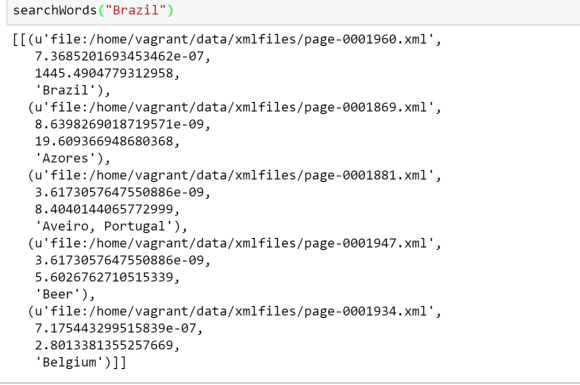
\includegraphics[width=5cm]{1} }}%
\end{figure}

The four values in the results are to be interpreted as follows:
\begin{enumerate}

\item Input file path of the search result which was stored as the key in our case.
\item Page Rank Value
\item TF-iDF value for the search string
\item Page title of the wiki page for easier cross-reference and verification.
\end{enumerate}


Another search result for a two-word search string:

\begin{figure}[H]%
	\centering
	\subfloat[Search results for search string "Black Forest"]{{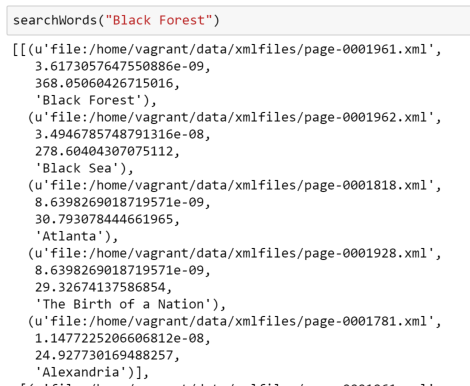
\includegraphics[width=5cm]{2} }}%
\end{figure}


\textbf{\underline{Note:}} Few other search results have been saved in a text file and have been attached with the project directory. Please check the folder named "Search Results" to see the other search results.
\newpage

\textbf{\underline{Future Work:}}

\begin{itemize}
	\item The open-endedness of the project allowed us the freedom to experiment with different approaches to determine which would work best for us. But for the lack of time, we could have experimented more with tf-idf and had a dictionary of values not just by per-word basis but also on different k-grams.
	
	\item There would be certain assumptions that we would have to consider, like saying the average search string length is 4 or 5 words and then computing and storing those corresponding k-grams.
	
	\item In that case, when a search string is provided, our code would look for a match for the k-gram and if there is a match, then our results would be even better. 
\end{itemize}

\end{document}